\documentclass[12pt]{article}
\usepackage[utf8]{inputenc}

\usepackage{enumitem}
\usepackage[margin=2cm]{geometry}

\usepackage{amsmath, amsfonts, amssymb}
\usepackage{graphicx}
\usepackage{tikz}
\usepackage{pgfplots}
\usepackage{multicol}

\usepackage{comment}
\usepackage{url}
\usepackage{calc}
\usepackage{subcaption}
\usepackage{circledsteps}

\usepackage{array}

\setlength\parindent{0pt}

\usepackage{fancyhdr}
\pagestyle{fancy}
\fancyhf{}
\renewcommand{\headrulewidth}{2pt}
\renewcommand{\footrulewidth}{0pt}
\rfoot{\thepage}
\lhead{\textsc{Math} 244}
\chead{\textsc{Homework 8}}
\rhead{Fall 2023}

\pgfplotsset{compat=1.16}

% MATH commands
\newcommand{\ga}{\left\langle}
\newcommand{\da}{\right\rangle}
\newcommand{\oa}{\left\lbrace}
\newcommand{\fa}{\right\rbrace}
\newcommand{\oc}{\left[}
\newcommand{\fc}{\right]}
\newcommand{\op}{\left(}
\newcommand{\fp}{\right)}

\newcommand{\bi}{\mathbf{i}}
\newcommand{\bj}{\mathbf{j}}
\newcommand{\bk}{\mathbf{k}}
\newcommand{\bF}{\mathbf{F}}

\newcommand{\ra}{\rightarrow}
\newcommand{\Ra}{\Rightarrow}

\newcommand{\sech}{\mathrm{sech}\,}
\newcommand{\csch}{\mathrm{csch}\,}
\newcommand{\curl}{\mathrm{curl}\,}
\newcommand{\dive}{\mathrm{div}\,}

\newcommand{\ve}{\varepsilon}
\newcommand{\spc}{\vspace*{0.5cm}}

\DeclareMathOperator{\Ran}{Ran}
\DeclareMathOperator{\Dom}{Dom}

\newcommand{\exo}[3]{\noindent\textcolor{red}{\fbox{\textbf{Section {#1}, Problem {#2}}}\hrulefill   \textbf{({#3} Pts})}\vspace*{10pt}}

\begin{document}
\thispagestyle{empty}
	\noindent \hrulefill \newline
	MATH-244 \hfill Pierre-Olivier Paris{\'e}\newline
	Homework 8 Solutions \hfill Fall 2023\newline \vspace*{-0.7cm}
	
	\noindent\hrulefill
	
	\spc

	\exo{16.2}{4}{5}
	\\
	A parametrization of the line segment is given by
		\[
			\vec{r} (t) = (1 - t) \left\langle 2, 0 \right\rangle + t \left\langle 5, 4, \right\rangle = \left\langle 2 + 3t , 4t \right\rangle \quad (0 \leq t \leq 1 ) .
		\]
	Therefore,
		\[
			\int_C xe^y \, ds = \int_0^1 (2 + 3t) e^{4t} \sqrt{3^2 + 4^2} \, dt = 5 \int_0^1 (2 + 3t ) e^{4t} \, dt = \frac{5}{16} (17 e^4 - 5) . \tag*{$\triangle$}
		\]

	\spc

	\exo{16.2}{8}{5}
	\\ 
	A parametrization of the circle $C_1$ of radius $2$ is
		\[
			\vec{r} (t) = \left\langle 2 \cos (t) , 2 \sin (t) \right\rangle \quad (0 \leq t \leq \pi / 2 )
		\]
	and a parametrization of the line segment $C_2$ is
		\[
			\vec{r} (t) = \left\langle 0, 2 \right\rangle + t (\left\langle 4, 3 \right\rangle - \left\langle 0, 2 \right\rangle ) = \left\langle 4t , 2 + t \right\rangle \quad (0 \leq t \leq 1 ) .
		\]
	Therefore, we have
		\begin{align*}
			\int_C x^2 \, dx + y^2 \, dy &= \int_{C_1} x^2 \, dx + y^2 \, dy + \int_{C_2} x^2 \, dx + y^2 \, dy \\ 
			&= \int_0^{\pi / 2} 4 \cos^2 (t) (-2 \sin (t)) \, dt + 4 \sin^2 (t) (2 \cos (t)) \, dt \\ 
			& \quad + \int_0^1 16 t^2 (4) \, dt + (1 + t)^2 \, dt \\ 
			&= 8 \int_0^{\pi / 2} \sin^2 (t) \cos (t) - \cos^2 (t) \sin (t) \, dt + \int_0^1 64 t^2 + (2 + t)^2 \, dt \\ 
			&= 0 + \frac{83}{3} \approx 27.6667 \tag*{$\triangle$}
		\end{align*}

	\spc 

	\exo{16.2}{10}{5}
	\\ 
	A parametrization of a line segment is
		\[
			\vec{r} (t) = (1 - t )  \left\langle 3, 1, 2 \right\rangle + t \left\langle 1, 2, 5 \right\rangle = \left\langle 3 - 2t , 1 + t , 2 + 3t \right\rangle \quad (0 \leq t \leq 1 ) .
		\]
	Here, $\vec{r}\, ' (t) = \left\langle -2, 1, 3 \right\rangle$, so that $|\vec{r} \, ' (t)| = \sqrt{4 + 1 + 9} = \sqrt{14}$. Hence,
		\[
			\int_C y^2 z \, ds = \int_0^1 (1 + t)^2 (2 + 3t ) \sqrt{14} \, dt = \frac{107 \sqrt{14}}{12} \approx 33.3631 . \tag*{$\triangle$}
		\]

	\newpage

	\exo{16.2}{18}{5}
	\\ 
	To answer this question, it will be helpful to have the following formula for the inner product of two vectors:
		\[
			\langle \vec{a} , \vec{b} \rangle = |\vec{a}| |\vec{b}| \cos (\theta ) ,
		\]
	where $\theta$ is the angle between the two vectors $\vec{a}$ and $\vec{b}$. Both curves are also circles, so the derivative have a constant modulus equal to the radius of the circle. Let $A_1$ and $A_2$ be the radii of the circles $C_1$ and $C_2$ respectively. 

	\begin{description}
		\item[$\mathbf{C_1}$.] Let $\vec{r} (t)$ be a parametrization of the curve so that $|\vec{r}\,' (t)| = A_1$ for any $t$. Then, following the direction of the curve, we see that $\vec{F} (\vec{r} (t)) \cdot \vec{r} \, ' (t)$ is positive mostly for all positions on the curve, because the angle between $\vec{F} (\vec{r} (t))$ and $\vec{r} \, ' (t)$ is mostly between $0$ and $\pi/2$. Therefore, $\cos (\theta ) \geq 0$ along the curve and
			$$ 
			\vec{F} (\vec{r} (t)) \cdot \vec{r} \, ' (t) = | \vec{F} (\vec{r} (t))| A_1 \cos (\theta ) \geq 0 .
			$$ 
		In other words, the vector field $\vec{F}$ follows the direction of the curve $C_1$ most of the time.
		\item[$\mathbf{C_2}$.] Let $\vec{r} (t)$ be a parametrization of the curve. Then, following the direction of the curve, we see that $\vec{F} (\vec{r} (t)) \cdot \vec{r} \, ' (t)$ is globally negative. It seems to be zero, but the length of the vector in the vector field $\vec{F}$ grows as we move from the origin. For half of the circle $C_2$, we can see that the angle between $\vec{F}$ and $\vec{r}\,'$ is between $0$ and $\pi/2$, so there will be a positive contribution to the integral. However, on the other half of the circle $C_2$, we can observe a change in the angle between $\vec{F}$ and $\vec{r}\,'$. The angle is now between $\pi/2$ and $\pi$, which result in a negative inner product. Since the length of the vectors in the vector field along the second half of the circle $C_2$ is greater than the length of the vectors in the first half of the circle $C_2$, the result of the line integral is negative. In other words, it is harder to swim along the second half of the circle than on the first half, which results in loosing energy to swim along this path.
	\end{description}

	\spc 

	\exo{16.2}{20}{5} 
	\\ 
	The derivative of $\vec{r} (t)$ is
		\[
			\vec{r} \, ' (t) = \left\langle 2t, 3t^2, -2 \right\rangle \quad (0 < t < 2 ) .
		\]
	Therefore, we get
		\begin{align*}
			\int_C \vec{F} \cdot d \vec{r} &= \int_0^2 \left\langle t^2 + t^6, -2t^3 , t^3 - 2t \right\rangle \cdot \left\langle 2t, 3t^2, -2 \right\rangle \, dt \\ 
			&= \int_0^2 2t^3 + 2t^7- 6 t^5 - 2t^3 + 4t \, dt \\ 
			&= \int_0^2 2t^7 - 6t^5 + 4t \, dt \\ 
			&= 8 . \tag*{$\triangle$}
		\end{align*}

	\spc 

	\exo{16.2}{22}{10} 
	\\ 
	The derivative of $\vec{r}(t)$ is
		\[
			\vec{r} \, ' (t) = \langle -\sin t , \cos t , 1 \rangle \quad (0 < t < \pi ) .
		\]
	Therefore, we get
		\begin{align*}
			\int_C  \vec{F} \cdot d\vec{r} &= \int_0^\pi \left\langle \cos t , \sin t , \cos t \sin t \right\rangle \cdot \left\langle -\sin t , \cos t , 1 \right\rangle \, dt \\ 
			&= \int_0^\pi -\sin t \cos t + \sin t \cos t + \cos t \sin t \, dt \\ 
			&= \int_0^\pi \cos t \sin t \, dt = 0 . \tag*{$\triangle$}
		\end{align*}

	\spc 

	\exo{16.2}{32}{10}
	\\ 
	\begin{enumerate}
		\item[(a)] The parametrization of the circle is $\vec{r} (t) = \left\langle 2 \cos t , 2 \sin t \right\rangle$, for $0 \leq t \leq 2\pi$. Therefore, $\vec{r} \, ' (t) = \left\langle -2\sin t , 2 \cos t \right\rangle$. Therefore,
			\begin{align*}
				\int_C \vec{F} \cdot d\vec{r} &= \int_0^{2\pi} \left\langle 4\cos^2 (t) , 4 \cos (t) \sin (t) \right\rangle \cdot \left\langle -2\sin t , 2 \cos t \right\rangle \, dt \\ 
				&= \int_0^{2\pi} -8 \cos^2 (t) \sin (t) + 8 \cos^2 (t) \sin (t) \, dt \\ 
				&= \int_0^{2\pi} 0 \, dt = 0 .
			\end{align*}
		\item[(b)] From the picture obtained using Python, we see that the line integral should be zero because the vector field is always perpendicular to the direction of the curve (the circle). Therefore, for every $t$, we have $\vec{F} \cdot \vec{r}\, ' = 0$. See the picture below.
		\begin{center}
		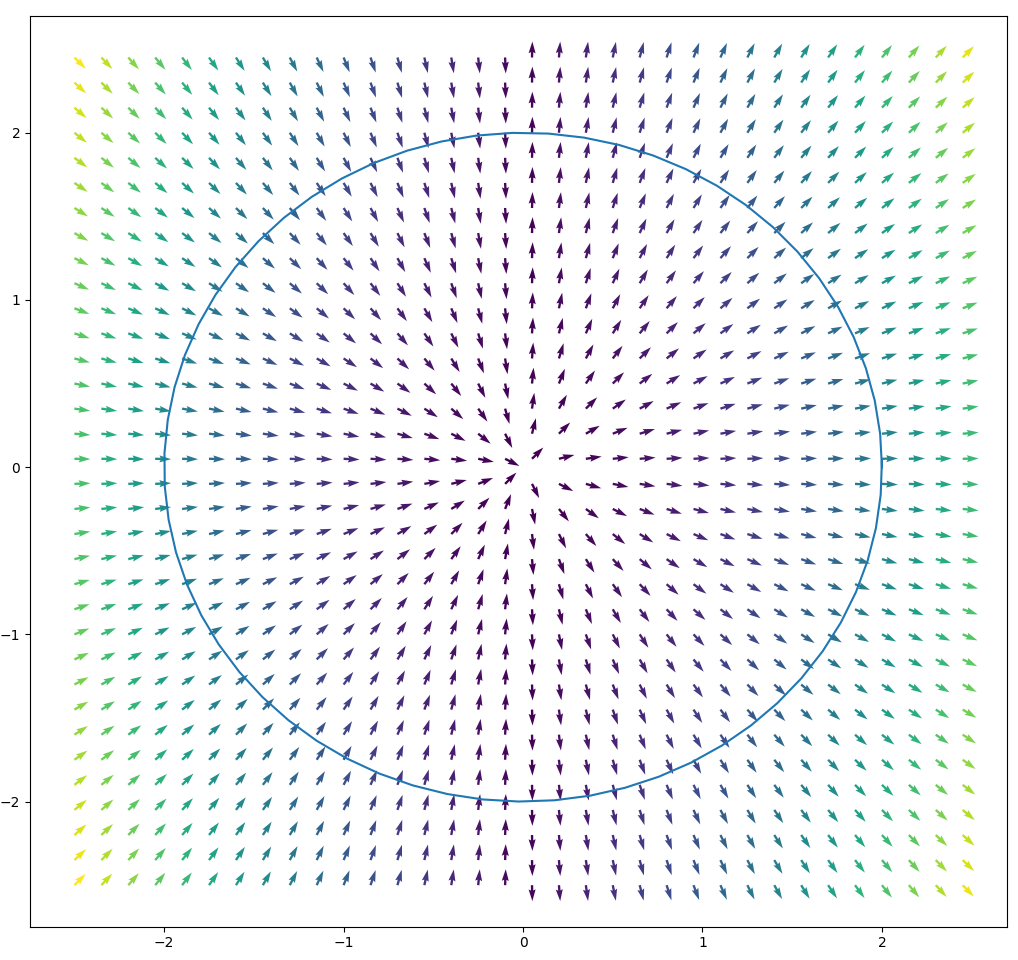
\includegraphics[scale=0.225]{prob32.png}
		\end{center}
	\end{enumerate}

	\spc 

	\exo{16.2}{50}{5}
	\\ 
	By definition, we have
		\[
			\int_C \vec{r} \cdot d \vec{r} = \int_a^b \vec{r} (t) \cdot \vec{r}\,' (t) \, dt .
		\]
	Recall from Chapter 13, the following property:
		\[
			\frac{d}{dt} ( \vec{u} (t) \cdot \vec{v} (t) ) = \vec{u}\,' (t) \cdot \vec{v} (t) + \vec{u} (t) \cdot \vec{v}\,'(t) ,
		\]
	where $\vec{u} (t)$ and $\vec{v}(t)$ are two vector-valued functions of the parameter $t$. With $\vec{u} = \vec{v} = \vec{r}$, we see that
		\[
			\frac{d}{dt} (|\vec{r}(t)|^2) = 2 \vec{r} (t) \cdot \vec{r} \, ' (t) .
		\]
	Therefore, plugging that in the expression of the line integral, we get
		\[
			\int_C \vec{r} \cdot d \vec{r} = \frac{1}{2}  \int_a^b \frac{d}{dt} ( |\vec{r} (t)|^2 ) \, dt = 
			= \frac{1}{2} \left. \Big( |\vec{r} (t)|^2 \Big) \right|_a^b 
			= \frac{1}{2} (|\vec{r} (b)|^2 - |\vec{r} (a)|^2 ) . \tag*{$\triangle$}
		\]


	\vfill

\hfill \textsc{Total:} 50 Pts.
	
	
	
\end{document}